\subsubsection{Tokens and semantic interpretation.}

Inspecting activating tokens and their surrounding text helps formulate semantic interpretations of sparse features~\cite{bricken2023monosemanticity}. We examine the original failing programs in the selected cohorts: 119 DeepSeek base outputs for feature 4810 and 50 CodeLlama merged outputs for feature 4309. All token statistics below refer to these programs. Figure~\ref{fig:case-token-contexts} summarizes their activating-token profiles through clouds weighted by summed positive activation, rather than frequency-controlled token associations.

\begin{figure*}[t]
\centering
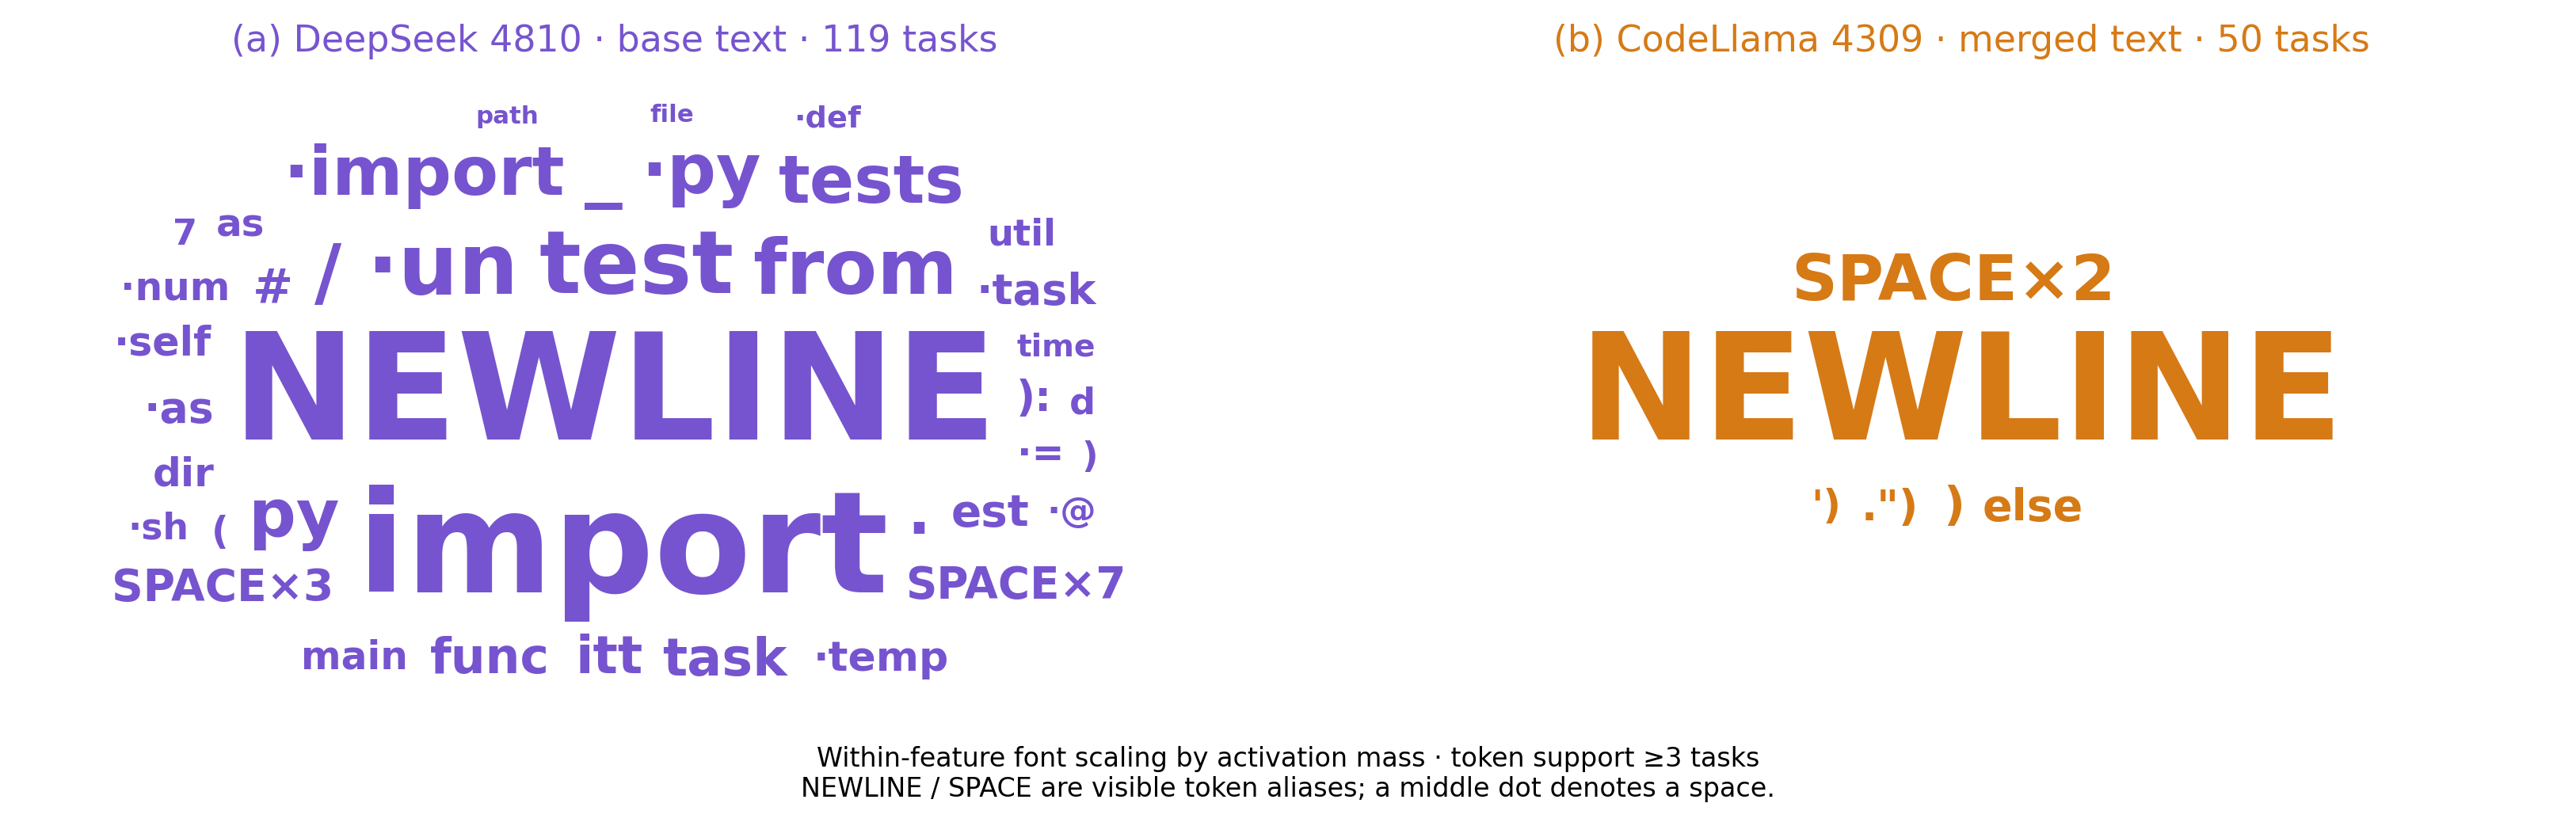
\includegraphics[width=\textwidth]{emse-submission/crosscoder_case_studies/figures/feature_token_clouds.png}
\caption{Activating-token clouds for DeepSeek 4810 on 119 original failing base programs (purple) and CodeLlama 4309 on 50 original failing merged programs (orange). Font size increases with the square root of summed activation mass within each feature. Displayed token IDs require activation in at least three tasks; up to 40 are selected per feature. \texttt{NEWLINE} and \texttt{SPACE} are visible aliases, and a middle dot denotes a space. Font scales are independent across features.}
\label{fig:case-token-contexts}
\end{figure*}

For DeepSeek, prominent activating tokens include \texttt{import}, \texttt{from}, \texttt{test}, filename fragments, and newlines. This profile is consistent with test-like or illustrative code continuation, rather than uniquely identifying invalid imports. For CodeLlama, newline tokens account for 80.8\% of feature 4309's activation mass, making the preceding line context particularly relevant to its interpretation.

We therefore further inspect the lines ending at the 141 CodeLlama newline tokens with positive activation (Figure~\ref{fig:case-newline-contexts}). Of these, 49 end return statements (34.8\%), 28 end \texttt{raise} statements (19.9\%), 15 end block headers (10.6\%), 14 end assignments (9.9\%), 12 end blank lines (8.5\%), and 23 end other lines (16.3\%), including calls and \texttt{continue} statements. These percentages use the same denominator of 141 active newline occurrences throughout; they are not percentages of tasks.

\begin{figure}[t]
\centering
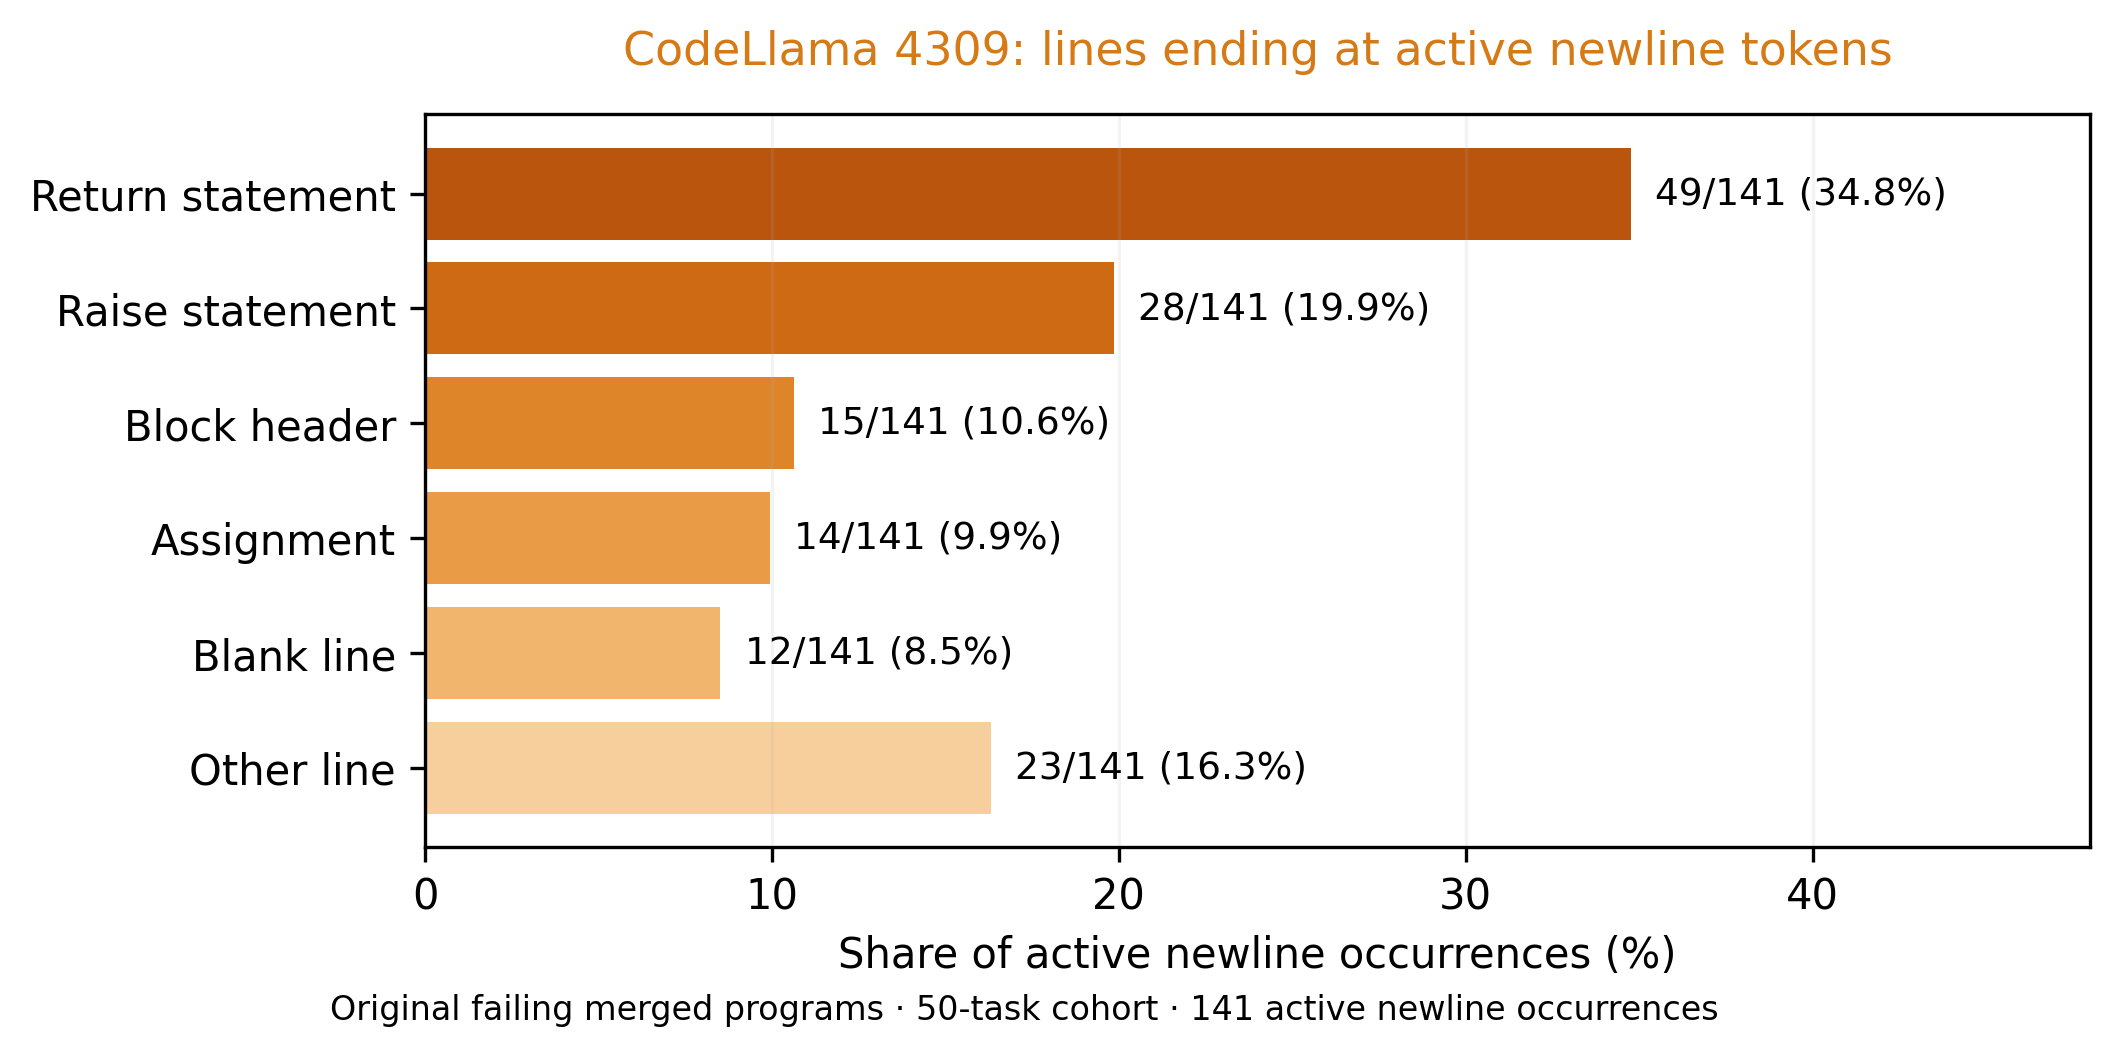
\includegraphics[width=\linewidth]{emse-submission/crosscoder_case_studies/figures/codellama_active_newline_contexts.png}
\caption{Line contexts for the 141 active newline occurrences in the 50 original failing CodeLlama merged programs. Each occurrence is assigned once to the physical line it ends. Return statements are identified from AST end lines inside \texttt{task\_func}; a return may be conditional and need not be the function's last return. Other categories distinguish \texttt{raise} statements, block headers, assignments, blank lines, and remaining lines. Counts pool token occurrences across tasks and are descriptive, not independent task-level observations.}
\label{fig:case-newline-contexts}
\end{figure}

Together, these contexts suggest that feature 4309 is associated with line and statement boundaries, including returns, rather than exclusively with return statements or erroneous code. The two token profiles provide complementary semantic hypotheses: test-like continuation for DeepSeek and structural boundaries for CodeLlama. They do not establish a unique feature meaning or, by themselves, a causal mechanism. The token statistics and line-level classifications are available in our replication package~\cite{CrossCoderReplication}.
